\documentclass[10pt]{article}
\usepackage{dfsha-informe}

\hito{2}
\title{DFSha: Arquitectura distribuida y comunicaciones}
\date{28 de septiembre de 2026}

\begin{document}
\portada

\textbf{Opción asignada:} Opción 1, Cliente/Servidor, con el servicio distribuido entre varios nodos dentro de una red privada.

Este informe parte de la especificación del Hito 1 y describe lo que se construyó en el Hito 2. Las decisiones se enuncian en el cuerpo y se justifican en las \textbf{Notas} del final. Las notas del Hito 1 se citan como \emph{Hito 1, N3}.

\textbf{Código fuente:} \url{https://github.com/AndresVelezR/DFSha---Distributed-Systems}, etiqueta \texttt{hito-2}.

\separador

% =============================================================================
\section{1. Objetivo y alcance}

\subsection{Objetivo}

Convertir la especificación del Hito 1 en un sistema que corre. Un cliente, un ControlNode y varios DataNodes se comunican por red: los archivos se parten en bloques, los bloques se reparten y se replican entre DataNodes, y los datos nunca pasan por el ControlNode. Además, dejar fijado el contrato de comunicación de todas las relaciones entre componentes, incluidas las que se implementan en el Hito 3.

\subsection{Marco teórico}

Un sistema de archivos distribuido guarda archivos repartidos en varias máquinas y permite accederlos como si fueran un solo sistema. Hay dos enfoques. En el almacenamiento por objetos, como S3, la unidad es el archivo completo. En el almacenamiento por bloques, como GFS y HDFS, el archivo se parte y cada parte se ubica por separado. DFSha es por bloques porque el enunciado pide que cada archivo quede repartido entre varios nodos y que haya concurrencia dentro de un mismo archivo (Hito 1, N1).

De GFS y HDFS se toman dos ideas. La primera es separar el plano de control del plano de datos. Un nodo maestro guarda solo metadatos y decide dónde va cada bloque, y los datos viajan directamente entre el cliente y los nodos de almacenamiento, así que el maestro no se vuelve cuello de botella con archivos grandes. La segunda es la escritura única: los bloques no se modifican nunca, así que dos copias de un bloque son idénticas por construcción y no hay que reconciliar réplicas (Hito 1, N8). Todo lo demás se construye desde cero; no se instala ni se envuelve Hadoop.

\subsection{Alcance}

El cronograma del curso asigna al Hito 2 el diseño e implementación de la arquitectura distribuida y la especificación de comunicaciones, y al Hito 3 la alta disponibilidad, la replicación, la consistencia y la seguridad. La tabla muestra qué cubre este hito de cada criterio de evaluación.

\begin{xltabular}{\linewidth}{@{}L{4.3cm}Y@{}}
\toprule
Criterio & En el Hito 2 \\
\midrule\endhead
Definición del servicio y diseño arquitectónico & Arquitectura maestro--trabajador ejecutable con un ControlNode y tres DataNodes, más un cuarto opcional (sección 2) \\
Especificaciones de comunicaciones & Contrato de las cinco relaciones entre componentes, con errores y reintentos. Cuatro están implementadas; la de ControlNode con ControlNode queda definida (sección 4) \\
Diseño para escalabilidad & DataNodes que se agregan con el sistema en marcha, tamaño de bloque que se adapta al número de nodos y ubicación por ocupación (secciones 3 y 6) \\
Replicación y consistencia & Réplica de bloques entre DataNodes, escritura única y un solo escritor por archivo. La réplica de metadatos y la reparación de copias son del Hito 3 \\
Alta disponibilidad & Lectura desde otra réplica cuando un DataNode falla. Los tres ControlNodes y la reparación automática son del Hito 3 \\
Seguridad & Token del cliente y clave compartida del clúster. HTTPS, cifrado y usuarios reales son del Hito 3 \\
\bottomrule
\end{xltabular}

\separador

% =============================================================================
\section{2. Arquitectura implementada}

\textbf{Tipo de arquitectura: Maestro y Trabajador}, la definida en el Hito 1. El ControlNode coordina y sabe dónde está todo, y los DataNodes guardan los datos. El cliente le pide un plan al ControlNode y mueve los bloques directamente con los DataNodes.

\begin{figure}[htbp]
\centering
\begin{tikzpicture}
  \node[caja, minimum width=2.4cm] (cli) at (0,-2.6) {Cliente\\\footnotesize CLI en Python};
  \node[caja, minimum width=3.4cm] (cn) at (7.4,1.0) {ControlNode cn-01\\\footnotesize Go, puerto 8000};
  \node[cajaclara, minimum width=2.6cm] (cnr) at (11.4,1.0) {cn-02 y cn-03\\\footnotesize Hito 3};
  \node[caja, minimum width=3.2cm] (dn1) at (7.4,-1.3) {DataNode dn-01\\\footnotesize Go, puerto 8001};
  \node[caja, minimum width=3.2cm] (dn2) at (7.4,-2.6) {DataNode dn-02};
  \node[caja, minimum width=3.2cm] (dn3) at (7.4,-3.9) {DataNode dn-03};
  \node[cajaclara, minimum width=3.2cm] (dn4) at (7.4,-5.2) {DataNode dn-04\\\footnotesize se agrega en caliente};
  \coordinate (espacioreplica) at ($(dn2.east)+(1.3,0)$);
  \node[draw, gray!60, rounded corners=3pt, inner sep=7pt,
        fit=(dn1)(dn4)(espacioreplica)] (dns) {};

  \draw[flecha] (cli.north) |- node[pos=0.75, above, font=\footnotesize] {REST/JSON: planes y metadatos} (cn.west);
  \draw[flecha] (cli.east) -- node[above, sloped, font=\footnotesize] {REST/binario: bloques} (dn1.west);
  \draw[flecha] (cli.east) -- (dn2.west);
  \draw[flecha] (cli.east) -- (dn3.west);
  \draw[flechaclara] (cli.east) -- (dn4.west);
  \draw[flecha] (dns.north) -- node[right, font=\footnotesize] {registro y heartbeat} (cn.south);
  \draw[flechaclara] (cn.east) -- (cnr.west);
  \draw[flecha] (dn1.east) to[bend left=55] (dn2.east);
  \draw[flecha] (dn2.east) to[bend left=55] node[right, font=\footnotesize, align=left] {réplica\\entre\\DataNodes} (dn3.east);
\end{tikzpicture}
\end{figure}

En este hito hay un solo ControlNode activo. En el diagrama, los otros dos del diseño del Hito 1 aparecen en punteado: su réplica de metadatos y la elección de líder son del Hito 3, y sus endpoints ya existen y responden \texttt{501}. El cuarto DataNode está apagado por defecto y sirve para demostrar el escalado.

\subsection{Componentes}

\begin{itemize}
\item \textbf{Cliente} (Python, sin dependencias externas). Programa de línea de comandos que se autentica, ejecuta los comandos del sistema de archivos, parte los archivos al subirlos y los reconstruye al bajarlos. No tiene direcciones de DataNodes en su configuración: las recibe en cada plan (Hito 1, N6).
\item \textbf{ControlNode} (Go). Guarda en memoria el árbol de directorios, los metadatos de cada archivo y la lista de DataNodes con su ocupación. Calcula los planes de escritura y lectura, y publica un archivo solo cuando todos sus bloques se subieron.
\item \textbf{DataNode} (Go). Guarda los bloques en su disco, verifica la firma de cada uno al recibirlo, los entrega completos o por rangos de bytes y los propaga a otros DataNodes. Se registra solo al arrancar y manda un heartbeat periódico con su ocupación.
\end{itemize}

\subsection{Organización del código}

Cada nodo es un binario independiente. Dentro de cada uno, el código se separa en archivos por responsabilidad, de modo que cada archivo tiene un solo motivo para cambiar \vernota{N1}.

\begin{xltabular}{\linewidth}{@{}L{5.2cm}Y@{}}
\toprule
Archivo & Responsabilidad \\
\midrule\endhead
\texttt{controlnode/config.go} & Parámetros operativos, leídos de variables de entorno y validados al arrancar \\
\texttt{controlnode/planner.go} & Decisiones de particionamiento y ubicación: tamaño de bloque, número de copias, capacidad y destinos. No depende de HTTP \\
\texttt{controlnode/handlers\_*.go} & Endpoints agrupados por tema: autenticación, sistema de archivos, subida, descarga y clúster \\
\texttt{controlnode/server.go} & Estado en memoria y tabla de rutas \\
\texttt{datanode/handlers.go} & Endpoints de bloques \\
\texttt{datanode/control\_client.go} & Comunicación con el ControlNode: registro y heartbeat \\
\texttt{datanode/peer\_client.go} & Comunicación con otros DataNodes: propagación de copias \\
\texttt{datanode/storage.go} & Disco local: capacidad, bloques guardados y bytes que ocupan \\
\texttt{client/dfsha.py} & Cliente de línea de comandos \\
\bottomrule
\end{xltabular}

\separador

% =============================================================================
\section{3. Algoritmos de particionamiento y distribución}

Las decisiones de esta sección viven en \texttt{planner.go} como funciones puras y tienen pruebas automáticas (sección 6).

\subsection{Tamaño de bloque}

Se implementa la fórmula del Hito 1 (N3), con los parámetros leídos de la configuración:

\begin{codigo}
B = clamp( block_size_min , S / (k · N) , block_size_max )
\end{codigo}

donde \texttt{S} es el tamaño del archivo, \texttt{N} el número de DataNodes vivos y \texttt{k} los bloques mínimos por nodo, redondeando a la potencia de dos inferior. Con los valores por defecto (8 MiB, 64 MiB y \texttt{k = 4}):

\begin{xltabular}{\linewidth}{@{}YYYYY@{}}
\toprule
Archivo & Bloque con 3 nodos & Bloques & Bloque con 4 nodos & Bloques \\
\midrule\endhead
1 MB & 8 MiB & 1 & 8 MiB & 1 \\
40 MB & 8 MiB & 5 & 8 MiB & 5 \\
200 MB & 8 MiB & 24 & 8 MiB & 24 \\
500 MB & 32 MiB & 15 & 16 MiB & 30 \\
1 GiB & 64 MiB & 16 & 64 MiB & 16 \\
10 GiB & 64 MiB & 160 & 64 MiB & 160 \\
\bottomrule
\end{xltabular}

La fila de 500 MB muestra la adaptación al clúster: con un nodo más, el bloque se reduce a la mitad para que cada nodo siga recibiendo al menos \texttt{k} bloques.

\subsection{Número de copias}

Se aplican las dos reglas del Hito 1 (N4 y ``Qué pasa al quitar un nodo''), en este orden:

\begin{enumerate}
\item El factor configurado nunca supera \texttt{N - 1}, donde \texttt{N} es el número de DataNodes registrados en el clúster, para que siempre exista un nodo donde rehacer una copia perdida \vernota{N2}.
\item Si hay menos DataNodes vivos que ese factor, se guardan las copias posibles en vez de rechazar la escritura, y el ControlNode lo avisa en su registro.
\end{enumerate}

\begin{xltabular}{\linewidth}{@{}YYYY@{}}
\toprule
Registrados & Vivos & Factor configurado & Copias por bloque \\
\midrule\endhead
3 & 3 & 2 & 2 \\
3 & 2 & 2 & 2 \\
3 & 1 & 2 & 1, con aviso \\
2 & 2 & 2 & 1 \\
3 & 3 & 3 & 2 \\
10 & 10 & 3 & 3 \\
\bottomrule
\end{xltabular}

Las copias de un mismo bloque siempre quedan en DataNodes distintos.

\subsection{Ubicación de los bloques}

Se usa la asignación voraz al nodo menos cargado, el \emph{list scheduling} de Graham (Hito 1, N5). Para cada copia de cada bloque se elige el DataNode vivo con menor porcentaje de ocupación que no tenga ya una copia de ese bloque. La implementación agrega tres detalles:

\begin{itemize}
\item \textbf{Carga virtual.} Mientras se arma el plan, a cada nodo elegido se le suma el tamaño del bloque, para que los bloques de una misma subida no caigan todos en los nodos que estaban más vacíos al empezar \vernota{N3}.
\item \textbf{Desempate por identificador} de nodo, para que el mismo estado produzca siempre el mismo plan \vernota{N3}.
\item \textbf{Ocupación medida por bloques.} Cada DataNode reporta los bytes que ocupan sus bloques sobre la capacidad de su volumen, y no el espacio usado del disco \vernota{N4}.
\end{itemize}

\subsection{Capacidad}

Antes de entregar un plan, el ControlNode comprueba que el archivo, multiplicado por su número de copias, quepa en el espacio libre sumado de los DataNodes vivos. Si no cabe, responde \texttt{507} y no reserva la ruta, en vez de dejar que la subida falle a mitad de camino (Hito 1, ``Sobre el tamaño máximo de archivo'').

\subsection{Integridad e idempotencia}

Cada bloque se identifica por la firma SHA-256 de su contenido. El DataNode recalcula la firma al recibirlo y lo rechaza si no coincide. Lo escribe primero a un archivo temporal y lo renombra al final, así que nunca queda visible un bloque a medias. Al descargar, el cliente vuelve a verificar la firma de cada bloque.

Subir un bloque es idempotente: si el DataNode ya lo tiene, no lo reescribe, pero sí lo propaga a los destinos indicados \vernota{N5}.

\subsection{Un solo escritor por archivo}

Pedir un plan de subida reserva la ruta durante \texttt{write\_lease\_ttl}, que es de 60 s por defecto. Mientras la reserva esté vigente, otro plan sobre la misma ruta recibe \texttt{409}. Si el cliente muere, la reserva vence sola. El archivo solo se publica cuando el cliente confirma todos sus bloques, así que un archivo a medio subir nunca es visible (Hito 1, N8).

\subsection{Concurrencia y memoria}

El cliente sube y baja hasta cuatro bloques en paralelo (opción \texttt{-{}-workers}, Hito 1 N10), y cada DataNode atiende cada conexión en una goroutine. Cada worker lee del disco solo su bloque, y al bajar escribe cada bloque directamente en su posición del archivo de salida. Así, en memoria nunca hay más de \emph{workers $\times$ tamaño de bloque} bytes, sin importar el tamaño del archivo \vernota{N6}.

\separador

% =============================================================================
\section{4. Comunicaciones}

Todo es \textbf{REST sobre HTTP} (Hito 1, N11): el control viaja en JSON y los bloques como cuerpo binario sin codificar. El cliente envía su token en la cabecera \texttt{Authorization: Bearer} a todos los nodos, y los nodos entre sí se identifican con la clave del clúster en \texttt{X-Cluster-Key}. En este hito se usa HTTP; el contrato no cambia al activar HTTPS en el Hito 3. El ControlNode escucha en el puerto \textbf{8000} y cada DataNode en el \textbf{8001}.

\subsection{Protocolo por cada relación}

\begin{xltabular}{\linewidth}{@{}L{2.5cm}L{2.0cm}L{2.2cm}YY@{}}
\toprule
Relación & Expone & Protocolo & Para qué & Estado \\
\midrule\endhead
Cliente y ControlNode & ControlNode & REST/JSON & Autenticación, sistema de archivos, planes de escritura y lectura, confirmación & Implementada \\
Cliente y DataNode & DataNode & REST/binario & Subir y bajar bloques & Implementada \\
DataNode y DataNode & DataNode & REST/binario & Propagar la copia al escribir & Implementada \\
ControlNode y DataNode & ControlNode & REST/JSON & Registro, heartbeat y reporte de bloques & Implementada; las órdenes de reparación que viajan en la respuesta del heartbeat son del Hito 3 \\
ControlNode y ControlNode & ControlNode & REST/JSON & Réplica de metadatos y elección de líder & Contrato definido; responde \texttt{501} hasta el Hito 3 \\
\bottomrule
\end{xltabular}

\subsection{Errores y reintentos}

\begin{xltabular}{\linewidth}{@{}L{5.2cm}Y@{}}
\toprule
Situación & Comportamiento \\
\midrule\endhead
Fallo de red al subir un bloque & Hasta 3 reintentos contra el mismo DataNode, esperando 1, 2 y 4 s. Es seguro porque la operación es idempotente \vernota{N7} \\
Fallo al bajar un bloque, o firma incorrecta & Se pasa de inmediato a la siguiente réplica, sin reintentar la misma \\
Respuesta de error del servidor & No se reintenta: no es un fallo de red sino una decisión del servidor \\
La reserva venció antes de confirmar (\texttt{410}) & El cliente pide un plan nuevo y repite la subida una vez; los bloques ya subidos no se duplican \\
Un bloque sin copias vivas al pedir el plan de lectura & El ControlNode responde \texttt{503} \\
\bottomrule
\end{xltabular}

\subsection{API del ControlNode, la consume el cliente}

\begin{xltabular}{\linewidth}{@{}L{3.6cm}YYL{2.9cm}@{}}
\toprule
Operación & Solicitud & Respuesta & Errores \\
\midrule\endhead
\texttt{POST} \ruta{/auth/login} & \texttt{\{username, password\}} & \texttt{200 \{token, expires\_in\}} & \texttt{401} \\
\texttt{GET} \ruta{/fs/ls?path=} & sin cuerpo & \texttt{200 \{entries:[\{name, type, size, blocks, replicas\_ok\}]\}} & \texttt{404} \\
\texttt{POST} \ruta{/fs/mkdir} & \texttt{\{path\}} & \texttt{201} & \texttt{409} ya existe, \texttt{404} sin padre \\
\texttt{DELETE} \ruta{/fs/rmdir?path=} & sin cuerpo & \texttt{204} & \texttt{409} no vacío, \texttt{404} \\
\texttt{DELETE} \ruta{/fs/rm?path=} & sin cuerpo & \texttt{204} & \texttt{404} \\
\texttt{POST} \ruta{/fs/mv} & \texttt{\{src, dst\}} & \texttt{200} & \texttt{404}, \texttt{409} destino existe \\
\texttt{GET} \ruta{/fs/stat?path=} & sin cuerpo & \texttt{200 \{size, block\_size, n\_blocks, replicas\_ok, owner\}} & \texttt{404} \\
\texttt{POST} \ruta{/files/upload/plan} & \texttt{\{path, size\}} & \texttt{200} con el plan de escritura & \texttt{409} reserva activa, \texttt{507} sin espacio, \texttt{404} sin padre, \texttt{503} sin DataNodes \\
\texttt{POST} \ruta{/files/upload/commit} & \texttt{\{upload\_id, blocks:[\{index, block\_id, size, stored\_on\}]\}} & \texttt{200 \{status:"publicado"\}} & \texttt{409} faltan bloques, \texttt{410} reserva vencida \\
\texttt{POST} \ruta{/files/upload/abort} & \texttt{\{upload\_id\}} & \texttt{204} & ninguno \\
\texttt{GET} \ruta{/files/download/plan?path=} & sin cuerpo & \texttt{200} con el plan de lectura y las réplicas vivas & \texttt{404}, \texttt{503} bloque sin copias \\
\bottomrule
\end{xltabular}

\texttt{replicas\_ok} es el número de copias en DataNodes vivos del bloque menos replicado del archivo, así que baja apenas un DataNode deja de mandar heartbeat. Este es el plan de escritura del archivo de la demostración, con los destinos que asignó el ControlNode; el identificador de subida y la fecha son ilustrativos:

\begin{codigo}
POST /files/upload/plan  ->  { "path": "/demo/original.bin", "size": 40000000 }
200 OK
{ "upload_id": "3f9c2a7e5b1d4c08", "block_size": 8388608, "n_blocks": 5,
  "lease_expires_at": "2026-09-28T05:20:12Z",
  "blocks": [
    { "index": 0, "targets": [ {"node":"dn-01","host":"dn1","port":8001},
                               {"node":"dn-02","host":"dn2","port":8001} ] },
    { "index": 1, "targets": [ {"node":"dn-03","host":"dn3","port":8001},
                               {"node":"dn-01","host":"dn1","port":8001} ] },
    ... ] }
\end{codigo}

\subsection{API del DataNode}

\begin{xltabular}{\linewidth}{@{}L{3.3cm}L{2.1cm}YYL{2.2cm}@{}}
\toprule
Operación & La consume & Solicitud & Respuesta & Errores \\
\midrule\endhead
\texttt{PUT} \ruta{/blocks/{id}} & Cliente, DataNode & Cuerpo binario. Si hay que propagar, \texttt{X-Forward-To} con las URL de los otros destinos y \texttt{X-Forward-Node-i} con sus identificadores & \texttt{201} si lo creó, \texttt{200} si ya existía; \texttt{\{block\_id, size, stored\_on\}} & \texttt{401}, \texttt{409} firma incorrecta \\
\texttt{GET} \ruta{/blocks/{id}} & Cliente, DataNode & Opcionalmente \texttt{Range} & \texttt{200} binario, \texttt{206} parcial & \texttt{401}, \texttt{404} \\
\texttt{DELETE} \ruta{/blocks/{id}} & ControlNode & \texttt{X-Cluster-Key} & \texttt{204} & \texttt{401}, \texttt{404} \\
\texttt{POST} \ruta{/blocks/{id}/replicate} & ControlNode & \texttt{\{target:\{host, port\}\}} & \texttt{202} & \texttt{401}, \texttt{502} \\
\texttt{GET} \ruta{/health} & Operación & sin cuerpo & \texttt{200 \{node\_id, capacity, used, n\_blocks\}} & ninguno \\
\bottomrule
\end{xltabular}

\subsection{API interna del clúster}

\begin{xltabular}{\linewidth}{@{}L{4.1cm}L{3.3cm}Y@{}}
\toprule
Operación & Quién la usa & Para qué \\
\midrule\endhead
\texttt{POST} \ruta{/cluster/register} & DataNode $\rightarrow$ ControlNode & Alta al arrancar con \texttt{\{node\_id, host, port, capacity, used\}}. Se repite sola si el ControlNode deja de reconocer al nodo \\
\texttt{POST} \ruta{/cluster/heartbeat} & DataNode $\rightarrow$ ControlNode & Señal de vida cada 3 s con \texttt{\{node\_id, capacity, used\}}. La respuesta trae \texttt{\{orders:[]\}}, vacía hasta el Hito 3 \\
\texttt{POST} \ruta{/cluster/blockreport} & DataNode $\rightarrow$ ControlNode & Inventario \texttt{\{node\_id, blocks:[id]\}}. Contrato fijado; el DataNode lo empieza a enviar en el Hito 3 \\
\texttt{POST} \ruta{/cluster/replicate} & Entre ControlNodes & Réplica de metadatos. Responde \texttt{501} hasta el Hito 3 \\
\texttt{POST} \ruta{/cluster/election} & Entre ControlNodes & Elección de líder con \texttt{\{node\_id, log\_length\}}. Responde \texttt{501} hasta el Hito 3 \\
\bottomrule
\end{xltabular}

\subsection{Cómo funciona una subida}

\begin{center}
\begin{tikzpicture}
  \participante{0}{-9.2}{Cliente}
  \participante{5.4}{-9.2}{ControlNode}
  \participante{9.5}{-9.2}{DataNode A}
  \participante{13.1}{-9.2}{DataNode B}
  \mensaje{0}{5.4}{-1.0}{\texttt{POST /files/upload/plan \{path, size\}}}
  \mensaje[flechaclara]{5.4}{0}{-2.0}{200: \texttt{upload\_id}, tamaño de bloque y destinos\\409 si la ruta está reservada, 507 si no cabe}
  \draw[gray!70, rounded corners=2pt] (-1.4,-2.5) rectangle (14.55,-7.0);
  \node[anchor=north west, font=\footnotesize\itshape, text=gray!70!black, fill=white, inner sep=1pt] at (-1.35,-2.52) {por cada bloque, hasta 4 en paralelo};
  \mensaje{0}{9.5}{-3.4}{\texttt{PUT /blocks/\{sha256\}} con \texttt{X-Forward-To: B}}
  \mensaje{9.5}{13.1}{-4.3}{\texttt{PUT /blocks/\{sha256\}}}
  \mensaje[flechaclara]{13.1}{9.5}{-5.1}{201}
  \mensaje[flechaclara]{9.5}{0}{-5.9}{201 \texttt{stored\_on = [A, B]}}
  \node[anchor=west, font=\footnotesize\itshape, text=gray!70!black, fill=white, inner sep=1pt] at (0.15,-6.55) {si falla la red: reintento a los 1, 2 y 4 s};
  \mensaje{0}{5.4}{-7.8}{\texttt{POST /files/upload/commit}}
  \mensaje[flechaclara]{5.4}{0}{-8.8}{200 publicado\\410 si venció la reserva: plan nuevo}
\end{tikzpicture}
\end{center}

\begin{enumerate}
\item El cliente pide el plan indicando ruta y tamaño.
\item El ControlNode valida la ruta, comprueba que no esté reservada y que el archivo quepa, calcula tamaño de bloque, número de copias y destinos, y reserva la ruta. El archivo queda en curso, no publicado.
\item El cliente lee cada bloque del disco, calcula su firma y lo envía al primer destino, hasta cuatro en paralelo.
\item El DataNode verifica la firma, guarda el bloque y lo propaga en cadena al siguiente destino, para que el cliente suba cada bloque una sola vez (Hito 1, N12).
\item El cliente confirma la subida con la lista de bloques y dónde quedó cada copia.
\item El ControlNode publica el archivo. Si la subida se interrumpe, el cliente la aborta o la reserva vence, y el archivo nunca se publica.
\end{enumerate}

\subsection{Cómo funciona una descarga}

\begin{center}
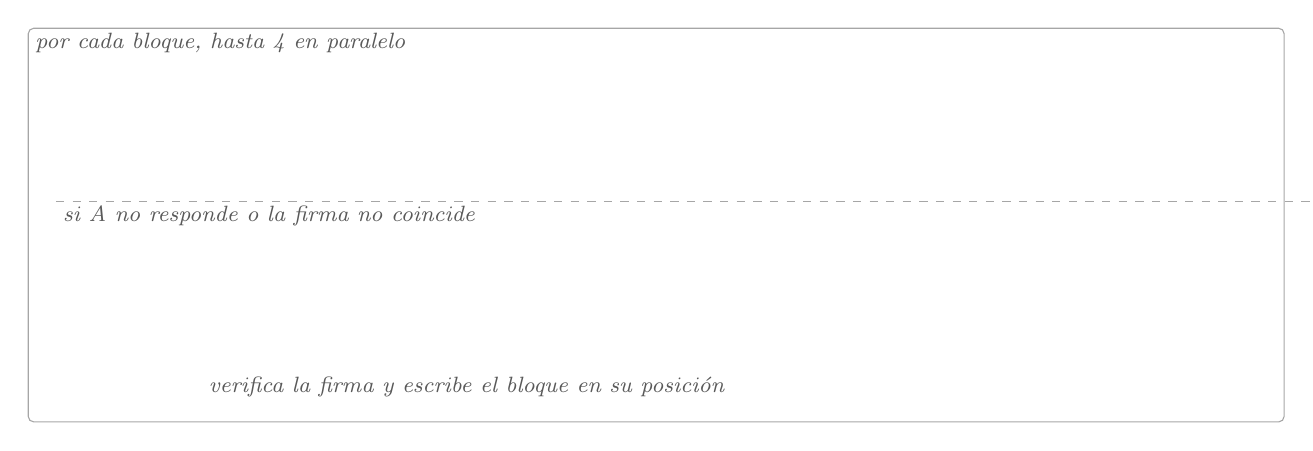
\begin{tikzpicture}
  \participante{0}{-7.9}{Cliente}
  \participante{5.4}{-7.9}{ControlNode}
  \participante{9.5}{-7.9}{DataNode A}
  \participante{13.1}{-7.9}{DataNode B}
  \mensaje{0}{5.4}{-1.0}{\texttt{GET /files/download/plan?path=}}
  \mensaje[flechaclara]{5.4}{0}{-2.0}{200: bloques y réplicas vivas\\503 si un bloque no tiene copias}
  \draw[gray!70, rounded corners=2pt] (-1.4,-2.5) rectangle (14.55,-7.5);
  \node[anchor=north west, font=\footnotesize\itshape, text=gray!70!black, fill=white, inner sep=1pt] at (-1.35,-2.52) {por cada bloque, hasta 4 en paralelo};
  \mensaje{0}{9.5}{-3.4}{\texttt{GET /blocks/\{sha256\}}}
  \mensaje[flechaclara]{9.5}{0}{-4.2}{bloque}
  \draw[gray!70, dashed] (-1.4,-4.7) -- (14.55,-4.7);
  \node[anchor=north west, font=\footnotesize\itshape, text=gray!70!black, fill=white, inner sep=1pt] at (-1.35,-4.72) {si A no responde o la firma no coincide};
  \mensaje{0}{13.1}{-5.6}{\texttt{GET /blocks/\{sha256\}}}
  \mensaje[flechaclara]{13.1}{0}{-6.4}{bloque}
  \node[anchor=west, font=\footnotesize\itshape, text=gray!70!black, fill=white, inner sep=1pt] at (0.15,-7.05) {verifica la firma y escribe el bloque en su posición};
\end{tikzpicture}
\end{center}

\begin{enumerate}
\item El cliente pide el plan de lectura.
\item El ControlNode devuelve, para cada bloque, las réplicas que están en DataNodes vivos.
\item El cliente descarga los bloques en paralelo. Si una réplica no responde o entrega una firma incorrecta, pasa a la siguiente.
\item Cada bloque verificado se escribe en su posición de un archivo temporal, que solo toma el nombre final cuando llegaron todos.
\end{enumerate}

\separador

% =============================================================================
\section{5. Entorno de ejecución}

Cada nodo corre en un contenedor Docker o de forma nativa, y expone su propia API REST. Hay tres formas de levantar el sistema, y las tres se probaron (sección 6).

\subsection{Docker Compose en una máquina}

\begin{xltabular}{\linewidth}{@{}L{3.2cm}YL{3.2cm}@{}}
\toprule
Servicio & Qué es & Puerto \\
\midrule\endhead
\texttt{controlnode} & ControlNode \texttt{cn-01} & 8000, publicado \\
\texttt{dn1}, \texttt{dn2}, \texttt{dn3} & DataNodes \texttt{dn-01} a \texttt{dn-03}, cada uno con su volumen & 8001, en la red interna \\
\texttt{dn4} & Cuarto DataNode, apagado por defecto (perfil \texttt{scale}) & 8001, en la red interna \\
\texttt{client} & Cliente, como herramienta (perfil \texttt{tools}) & ninguno \\
\bottomrule
\end{xltabular}

\begin{codigo}
docker compose up -d --build controlnode dn1 dn2 dn3
./scripts/demo.sh                       # demostración completa del hito
\end{codigo}

\subsection{Nativo}

\begin{codigo}
go build -o controlnode ./cmd/controlnode && ./controlnode
go build -o datanode ./cmd/datanode
NODE_ID=dn-01 PORT=8001 STORAGE_DIR=./dn1 ./datanode    # uno por DataNode
python3 client/dfsha.py login demo demo
\end{codigo}

\subsection{Varias máquinas en AWS Academy}

La infraestructura del Hito 1 (sección 5) queda preparada en la carpeta \texttt{deploy/aws} del repositorio: un solo archivo de Docker Compose para todas las VMs y un archivo \texttt{.env} por VM, que dice qué corre en ella y con qué dirección se anuncia a los demás.

\begin{xltabular}{\linewidth}{@{}L{2cm}Y@{}}
\toprule
VM & Contenedores en el Hito 2 \\
\midrule\endhead
vm-01 & ControlNode \texttt{cn-01} y DataNode \texttt{dn-01} \\
vm-02 & DataNode \texttt{dn-02}; \texttt{cn-02} se agrega en el Hito 3 \\
vm-03 & DataNode \texttt{dn-03}; \texttt{cn-03} se agrega en el Hito 3 \\
vm-04 & DataNode \texttt{dn-04}, apagada hasta la demostración de escalado \\
\bottomrule
\end{xltabular}

El puerto 8001 debe quedar abierto también hacia el cliente, porque el cliente sube y baja los bloques directamente de los DataNodes \vernota{N8}.

\subsection{Parámetros}

Todos los parámetros que usa la lógica implementada se leen de variables de entorno al arrancar, así que se cambian sin recompilar. Un valor inválido detiene el arranque con un mensaje que dice qué variable está mal.

\begin{xltabular}{\linewidth}{@{}L{4.1cm}L{4.8cm}L{1.3cm}Y@{}}
\toprule
Parámetro del Hito 1 & Variable de entorno & Defecto & Estado \\
\midrule\endhead
\texttt{replication\_factor} & \texttt{REPLICATION\_FACTOR} & 2 & Implementado \\
\texttt{block\_size\_min} & \texttt{BLOCK\_SIZE\_MIN\_MB} & 8 & Implementado \\
\texttt{block\_size\_max} & \texttt{BLOCK\_SIZE\_MAX\_MB} & 64 & Implementado \\
\texttt{blocks\_per\_node} & \texttt{BLOCKS\_PER\_NODE} & 4 & Implementado \\
\texttt{heartbeat\_interval} & \texttt{HEARTBEAT\_INTERVAL\_SECONDS} & 3 & Implementado \\
\texttt{heartbeat\_misses} & \texttt{HEARTBEAT\_MISSES} & 3 & Implementado: un nodo se da por muerto a los 9 s \\
\texttt{write\_lease\_ttl} & \texttt{WRITE\_LEASE\_TTL\_SECONDS} & 60 & Implementado \\
\texttt{client\_parallel\_blocks} & opción \texttt{-{}-workers} del cliente & 4 & Implementado \\
\texttt{availability\_target} & ninguna & & Ver el cambio 3 de la sección 7 \\
\texttt{node\_full\_threshold} & ninguna & & Hito 3, con el rebalanceo \\
\texttt{rebalance\_threshold} & ninguna & & Hito 3, con el rebalanceo \\
\texttt{blockreport\_interval} & ninguna & & Hito 3, con la reparación de copias \\
\texttt{cn\_heartbeat\_interval} & ninguna & & Hito 3, con los tres ControlNodes \\
\bottomrule
\end{xltabular}

No se exponen variables para funciones que todavía no existen, porque serían configuraciones sin efecto.

\separador

% =============================================================================
\section{6. Pruebas y análisis de resultados}

\subsection{Pruebas automáticas}

Se ejecutan con \texttt{go test ./...} y \texttt{python3 -m unittest discover client}. Solo usan la biblioteca estándar de cada lenguaje.

\begin{xltabular}{\linewidth}{@{}L{3.4cm}Y@{}}
\toprule
Qué se prueba & Casos \\
\midrule\endhead
Planificador & Tamaño de bloque (mínimo, máximo y redondeo), número de bloques, número de copias en los seis escenarios de la tabla de la sección 3, capacidad del clúster, copias en nodos distintos, reparto parejo y preferencia por el nodo más vacío \\
Endpoints de subida & Segunda reserva sobre la misma ruta: \texttt{409}. Reserva vencida: se libera. 3 DataNodes: 2 copias; 2 DataNodes: 1 copia. Archivo que no cabe: \texttt{507} sin dejar la ruta reservada \\
Sistema de archivos & \texttt{replicas\_ok} baja cuando un DataNode deja de mandar heartbeat \\
DataNode & La ocupación cuenta solo bloques completos, no escrituras en curso \\
Cliente & Reintentos a los 1 y 2 s hasta tener éxito; 4 intentos y luego falla; un error del servidor no se reintenta; un \texttt{410} pide un plan nuevo una sola vez; bloques escritos en desorden reconstruyen el archivo exacto \\
\bottomrule
\end{xltabular}

\subsection{Demostración de punta a punta}

\texttt{scripts/demo.sh} levanta el clúster con Docker Compose y ejecuta la secuencia completa. Resultado de la última ejecución:

\begin{xltabular}{\linewidth}{@{}L{4.6cm}Y@{}}
\toprule
Paso & Resultado \\
\midrule\endhead
Levantar el clúster & El ControlNode reporta 3 DataNodes vivos \\
Subir un archivo de 40 MB & 5 bloques de 8 MiB, cada uno con 2 copias en DataNodes distintos. \texttt{ls} y \texttt{stat} muestran \texttt{replicas\_ok: 2} \\
Descargarlo & Archivo reconstruido con la misma firma SHA-256 que el original \\
Dos planes seguidos sobre la misma ruta & \texttt{200} y luego \texttt{409} \\
Apagar \texttt{dn1} y descargar & A los 9 s el ControlNode reporta 2 DataNodes vivos. Los bloques que estaban en \texttt{dn-01} se leen de su otra réplica y la firma sigue siendo idéntica \\
Agregar \texttt{dn4} en caliente & El ControlNode pasa a 4 DataNodes vivos sin reiniciar nada. En la siguiente subida, \texttt{dn-04}, que llega vacío, recibe una copia de cada uno de los 5 bloques \\
\bottomrule
\end{xltabular}

\subsection{Pruebas de escenarios}

\begin{xltabular}{\linewidth}{@{}L{5.6cm}Y@{}}
\toprule
Escenario & Resultado \\
\midrule\endhead
Subida con un DataNode destino caído que vuelve a los 3 s & El cliente registra ``reintento 1/3 en 1s'' y ``reintento 2/3 en 2s'', y el bloque se sube en el tercer intento \\
3 DataNodes registrados y 1 caído & El plan asigna 2 copias por bloque entre los 2 vivos \\
Clúster de solo 2 DataNodes & El plan asigna 1 copia por bloque \\
\texttt{BLOCK\_SIZE\_MIN\_MB=4} al levantar & El bloque pasa a 4 MiB sin recompilar \\
\texttt{REPLICATION\_FACTOR=dos} & El ControlNode no arranca y reporta que el valor no es un entero \\
Tres VMs simuladas & Tres proyectos de Docker Compose sin red en común, con \texttt{deploy/aws} y cada DataNode en un puerto propio. Se comunican solo por la IP de la máquina, como entre VMs. El cliente nativo sube y baja un archivo de 30 MB y la firma coincide \\
Ejecución nativa & ControlNode y 3 DataNodes como procesos, sin Docker; subida y descarga correctas \\
\bottomrule
\end{xltabular}

\subsection{Medición de paralelismo}

Sobre las tres VMs simuladas se subió y bajó un archivo de 200 MB (24 bloques de 8 MiB, 2 copias) con 1 y con 4 workers, tres veces cada uno. La tabla muestra la mediana.

\begin{xltabular}{\linewidth}{@{}YYYYY@{}}
\toprule
Workers & Subida & Caudal de subida & Bajada & Caudal de bajada \\
\midrule\endhead
1 & 0.71 s & 280 MB/s & 0.57 s & 348 MB/s \\
4 & 0.36 s & 558 MB/s & 0.39 s & 513 MB/s \\
\bottomrule
\end{xltabular}

Con 4 workers la subida es 1.97 veces más rápida y la bajada 1.46 veces. La mejora confirma que el paralelismo por bloques funciona: mientras un bloque viaja, otro se lee y se firma. Los números absolutos no representan una red real, porque las tres VMs comparten una máquina y el tráfico no sale de ella. La medición sobre AWS queda para el Hito 4, como previó el Hito 1 (N10) \vernota{N9}.

\subsection{Análisis}

\begin{itemize}
\item \textbf{Separación de planos.} Los registros del ControlNode muestran solo peticiones de control. Los bloques viajan entre el cliente y los DataNodes, y entre DataNodes, así que el tamaño de los archivos no pasa por el ControlNode.
\item \textbf{Reparto.} En la subida de 40 MB, las 10 copias quedaron repartidas 4, 3 y 3 entre los tres DataNodes, y ningún bloque tuvo sus dos copias en el mismo nodo.
\item \textbf{Nodo nuevo.} Al agregar \texttt{dn-04}, las subidas nuevas lo prefieren hasta emparejar su ocupación. Es el autobalanceo por escrituras que describe el Hito 1: un nodo nuevo empieza a recibir bloques de inmediato, sin mover los que ya estaban guardados.
\item \textbf{Hallazgos corregidos durante las pruebas.} La primera ejecución del escalado no envió bloques a \texttt{dn-04} por dos causas. En Docker local los DataNodes medían su ocupación sobre el disco compartido de la máquina \vernota{N4}. Además, \texttt{dn4} usaba una imagen de Docker propia que no se reconstruía con las demás, así que corría código viejo. Ahora la ocupación se mide por bloques y todos los DataNodes comparten una imagen. También se corrigió que ejecutar el cliente con Docker Compose volvía a encender un DataNode apagado a propósito, lo que invalidaba la prueba de fallos \vernota{N10}.
\item \textbf{Copias degradadas.} Si la propagación de una copia falla durante la subida, por ejemplo porque el segundo destino se cae en ese momento, el bloque se publica con las copias que se lograron, como indica el Hito 1. \texttt{ls} y \texttt{stat} lo muestran en \texttt{replicas\_ok}, y reponer la copia faltante es trabajo de la reparación del Hito 3.
\end{itemize}

\separador

% =============================================================================
\section{7. Cambios respecto al Hito 1}

El Hito 1 previó que cualquier ajuste se documentaría en los hitos siguientes (RNF8). Estos son los cambios de decisión frente a lo planteado. Lo que simplemente se implementa en un hito posterior está en la sección 8.

\textbf{1. \texttt{cd} no se implementa como comando con estado de sesión.} El Hito 1 lo definió como un comando que maneja el cliente. El cliente construido no guarda estado: cada comando es un proceso nuevo y no hay una sesión que recuerde un directorio actual. La navegación se resuelve pasando la ruta completa a cada comando (\texttt{ls}, \texttt{stat}, \texttt{put}, \texttt{get}, \texttt{mv}). Cumple el mismo propósito sin agregar un estado local que se pueda desincronizar del servicio.

\textbf{2. Las primitivas de RF3 no se exponen como comandos ni endpoints separados.} \texttt{open}, \texttt{read} por rango, \texttt{write}, \texttt{lock} y \texttt{close} siguen siendo el modelo que fundamenta \texttt{put} y \texttt{get}. El plan de subida es el \texttt{open} con \texttt{lock}, porque reserva la ruta. Cada \texttt{PUT} de bloque es un \texttt{write}, y el commit es el \texttt{close}. El DataNode ya soporta lectura parcial con la cabecera \texttt{Range}. Exponerlas como superficie aparte no lo exige ningún criterio de este hito y agregaría una API que habría que mantener y asegurar en el Hito 3. Se reconsiderará si un hito posterior exige acceso aleatorio explícito a los archivos.

\textbf{3. Los parámetros se leen de variables de entorno, y \texttt{availability\_target} no se expone.} El Hito 1 pedía que ningún valor estuviera en el código y que se cambiaran sin recompilar, y eso se cumple. Las variables de entorno son el mecanismo nativo de Docker Compose, y un archivo \texttt{.env} junto al \texttt{docker-compose.yml} cumple el papel del archivo de configuración sin un formato adicional que leer y validar. El factor de replicación se configura directamente con el valor que da la fórmula de disponibilidad (Hito 1, N4). Recalcularlo en cada arranque no aporta nada, porque el resultado solo cambia cuando cambia el objetivo, que es justo cuando se ajusta la variable.

\textbf{4. Subir un bloque que ya existe responde \texttt{200}, no \texttt{409}.} El Hito 1 especificaba ``409 ya existe y se trata como éxito''. En HTTP, un \texttt{PUT} es idempotente y repetirlo con el mismo contenido es una operación exitosa, así que \texttt{200} describe mejor lo que pasa y evita que el cliente tenga que interpretar un código de error como éxito. Un bloque nuevo sigue respondiendo \texttt{201}.

\textbf{5. El puerto 8001 también se abre hacia el cliente.} La tabla de infraestructura del Hito 1 abría hacia el cliente solo el puerto 8000. Como el cliente sube y baja los bloques directamente de los DataNodes, también necesita el 8001 \vernota{N8}.

\separador

% =============================================================================
\section{8. Pendiente para el Hito 3}

Queda para el hito de Alta Disponibilidad, Replicación, Consistencia y Seguridad:

\begin{itemize}
\item \textbf{Tres ControlNodes} con réplica de metadatos y elección de líder. \ruta{/cluster/replicate} y \ruta{/cluster/election} responden \texttt{501}.
\item \textbf{Persistencia de metadatos} en disco. Hoy viven en memoria y se pierden si el ControlNode se reinicia.
\item \textbf{Reparación de copias.} El campo \texttt{orders} de la respuesta del heartbeat existe pero siempre va vacío, y el DataNode todavía no envía su inventario de bloques. Si un DataNode muere, o si falla la propagación de un bloque durante una subida, ese bloque se queda con menos copias hasta que exista la reparación.
\item \textbf{Verificación de copias en el commit.} Hoy el ControlNode confía en la lista \texttt{stored\_on} que reporta el DataNode. Contrastarla con el inventario de bloques es parte de la reparación.
\item \textbf{Rebalanceo} de bloques ya guardados al agregar un nodo, y \texttt{node\_full\_threshold}.
\item \textbf{Recolección de bloques huérfanos} tras \texttt{rm} o una subida abortada.
\item \textbf{Seguridad:} HTTPS, cifrado de bloques en disco y control de acceso real por usuario. Hoy hay un único usuario de demostración.
\item \textbf{Despliegue en AWS Academy} sobre las VMs del Hito 1, con la configuración ya preparada en \texttt{deploy/aws}.
\end{itemize}

\separador

% =============================================================================
\section{Notas}

\nota{N1}{Por qué archivos por responsabilidad y no capas} Cada servicio tiene unos cientos de líneas. Una arquitectura hexagonal, con puertos y adaptadores, agregaría interfaces con una sola implementación cada una, porque hoy no hay un segundo almacenamiento de metadatos ni un segundo transporte que intercambiar. Lo que sí hacía falta era poder probar las decisiones del sistema sin levantar un servidor, y eso se logra dejando el planificador como funciones puras en su propio archivo. El punto en que una interfaz sí se justifica es el Hito 3: cuando los metadatos pasen de memoria a un registro persistente y replicado, el acceso a ellos tendrá dos implementaciones reales.

\nota{N2}{Por qué el tope N - 1 cuenta nodos registrados y no vivos} El Hito 1 impone \texttt{N - 1} para que siempre quede un nodo donde rehacer una copia perdida, y eso es una propiedad del tamaño del clúster. Si se aplicara sobre los nodos vivos, con 3 DataNodes y uno caído el sistema guardaría una sola copia teniendo dos nodos disponibles. Bajaría la redundancia justo cuando ya ocurrió una falla, y contradiría la regla del mismo Hito 1 de que, con nodos caídos, se guardan las copias que se puedan.

\nota{N3}{Por qué carga virtual y desempate} La ocupación de cada nodo llega con el heartbeat cada 3 segundos, así que todos los bloques de un plan se deciden sobre la misma foto. Sin carga virtual, los 16 bloques de un archivo de 1 GiB irían a los mismos dos nodos, los más vacíos al empezar. Sumando el tamaño de cada bloque asignado, la heurística reparte dentro del mismo plan. El desempate por identificador existe porque Go recorre los mapas en orden aleatorio: sin él, dos nodos con la misma ocupación producirían planes distintos cada vez, lo que dificulta probar y explicar el sistema.

\nota{N4}{Por qué la ocupación se mide por bloques} El Hito 1 ubica cada bloque en el nodo con menor porcentaje de disco ocupado, y supone un volumen dedicado a bloques en cada VM. En ese volumen, el espacio usado del disco y los bytes de bloques coinciden. En Docker sobre una sola máquina, en cambio, todos los DataNodes ven el mismo disco, y el espacio usado refleja todo lo que hay en la máquina. En la prueba de escalado eso hizo que un nodo vacío pareciera tan lleno como los demás. Contar los bytes de los bloques da la medida correcta en ambos casos.

\nota{N5}{Por qué se propaga un bloque que ya existe} Antes, un DataNode que ya tenía el bloque respondía sin propagarlo. Un reintento después de una falla parcial, o un bloque con el mismo contenido en otro archivo, que por eso tiene el mismo identificador, quedaba registrado con una sola copia. Además, el DataNode ahora consume el cuerpo de la petición aunque no lo guarde, para que el cliente termine de enviarlo sin un error de conexión.

\nota{N6}{Por qué memoria acotada} La primera versión del cliente leía el archivo completo antes de subirlo y juntaba todos los bloques en memoria antes de escribirlos al bajar. Con un archivo de 10 GB en una instancia \texttt{t3.small}, que tiene 2 GB de memoria, eso es imposible, y contradice la idea central del Hito 1: un archivo grande nunca se carga completo en memoria. La descarga escribe sobre un archivo \texttt{.part} que se renombra al final, para que una descarga fallida nunca deje un archivo que parezca completo.

\nota{N7}{Por qué se reintenta la escritura y no la lectura} Así lo define el Hito 1, y tiene una razón. Al escribir, el plan tiene un único punto de entrada para cada bloque, el primer destino, así que la única forma de insistir es reintentar ese mismo destino. Al leer hay varias réplicas, y pasar a la siguiente es más rápido que esperar 1, 2 y 4 segundos a la misma. Solo se reintentan los fallos de red, en los que no hubo respuesta. Una respuesta de error del servidor es una decisión, no un fallo pasajero, y repetirla daría el mismo resultado.

\nota{N8}{Por qué el puerto 8001 se abre hacia el cliente} La separación de planos, que es el centro de la arquitectura, exige que el cliente hable directamente con los DataNodes. Con el 8001 cerrado hacia el cliente, solo podrían subirse archivos desde dentro de la red de AWS. Por la misma razón, cada DataNode se anuncia con la dirección que el cliente puede alcanzar: la IP privada si el cliente corre dentro de la red de AWS, y la pública si corre desde fuera.

\nota{N9}{Por qué la medición es solo indicativa} En una sola máquina, las transferencias no cruzan una red real y compiten por el mismo procesador y el mismo disco. Sirve para confirmar que el paralelismo reduce el tiempo, pero no para dimensionar el sistema. Ajustar \texttt{client\_parallel\_blocks} con datos reales requiere las VMs de AWS.

\nota{N10}{Por qué el cliente de Docker no depende de los nodos} Docker Compose enciende las dependencias de un servicio cada vez que se ejecuta. Con el cliente declarado como dependiente de los DataNodes, ejecutarlo después de apagar uno lo volvía a encender, y la prueba de tolerancia a fallos no probaba nada. El cliente es una herramienta que se usa con el clúster ya levantado, así que no declara dependencias.

\separador

\section{Referencias}

\begin{itemize}
\item S. Ghemawat, H. Gobioff y S.-T. Leung. \emph{The Google File System}. ACM Symposium on Operating Systems Principles, 2003.
\item K. Shvachko, H. Kuang, S. Radia y R. Chansler. \emph{The Hadoop Distributed File System}. IEEE Symposium on Mass Storage Systems and Technologies, 2010.
\item R. L. Graham. \emph{Bounds for certain multiprocessing anomalies}. Bell System Technical Journal, 45(9), 1966.
\item A. Vélez Rendón y J. L. Restrepo. \emph{DFSha: Especificación del proyecto}, Hito 1, 2026. En \texttt{docs/hito-1}.
\end{itemize}

\end{document}
